\begin{frame}{Safety, Ethics Control}
  \begin{center}
    \Huge Safety, Ethics Control
  \end{center}
\end{frame}

\begin{frame}{Safety in Agentic Systems}
  \begin{itemize}
    \item[\textcolor{red}{$\triangleright$}] \textbf{Risks:}
    \begin{itemize}
      \item Autonomous actions without human oversight
      \item Errors in tool or API use
      \item Prompt injection or goal hijacking
      \item Recursive self-improvement without constraints
    \end{itemize}
    \vspace{1em}
    \item[\textcolor{red}{$\triangleright$}] \textbf{Mitigations:}
    \begin{itemize}
      \item Approval-based execution (human-in-the-loop)
      \item Guardrails and policy enforcement
      \item Explainability (XAI) for agent decisions
    \end{itemize}
  \end{itemize}
\end{frame}

\begin{frame}{Safety in Agentic Systems}
  \centering
  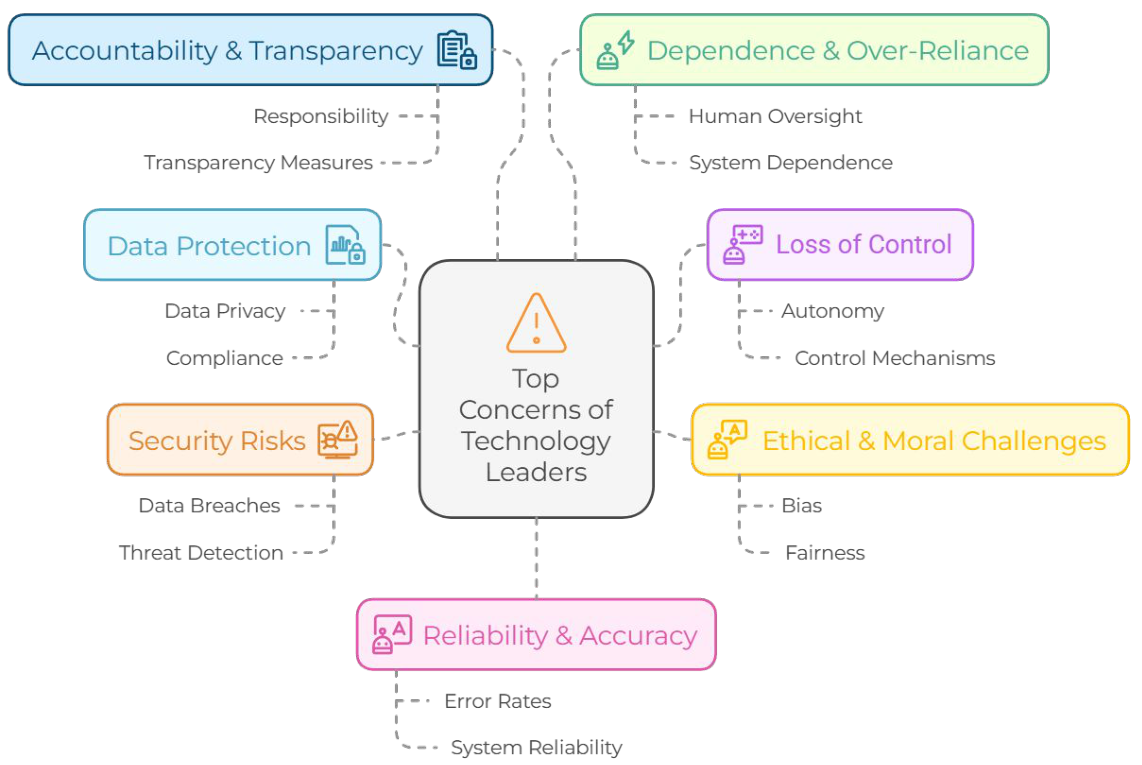
\includegraphics[width=0.8\textwidth,height=0.8\textheight,keepaspectratio]{assets/Lecture-10_Multimodal_NLP_Agentic_AI/slide_063.png}
\end{frame}

\begin{frame}{Safety in Agentic Systems}
  \begin{center}
    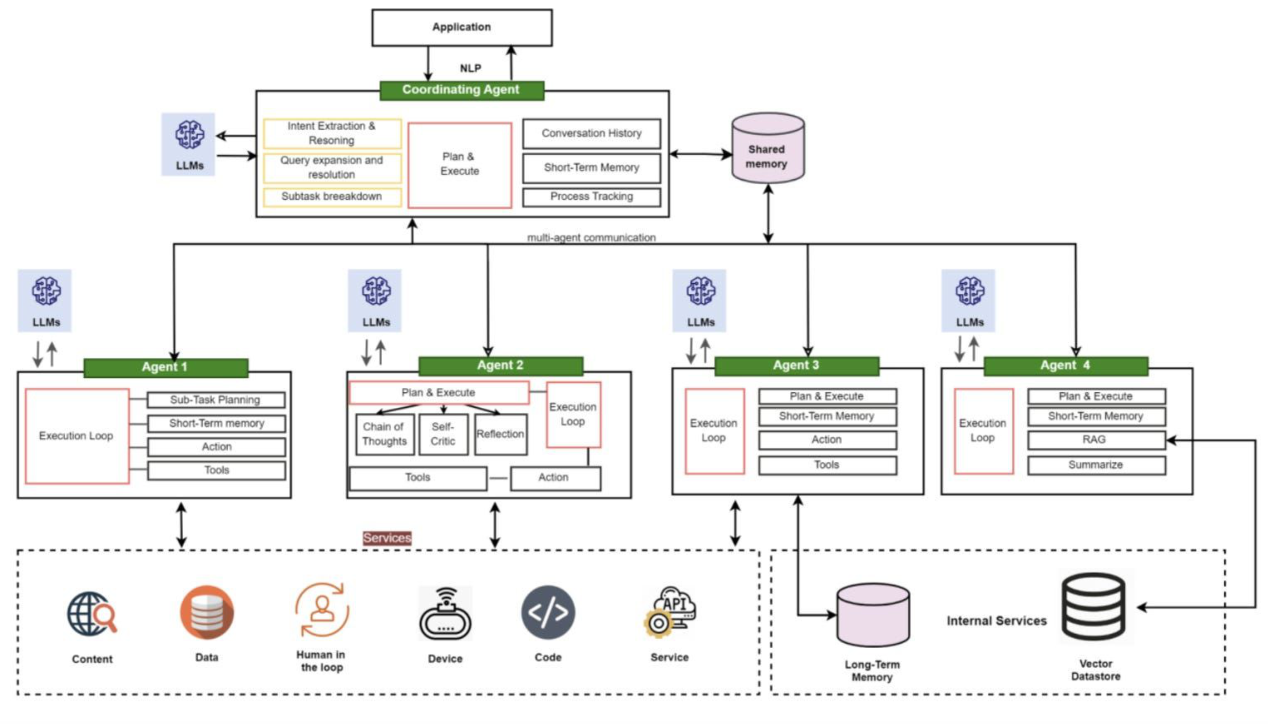
\includegraphics[width=0.8\textwidth,height=0.8\textheight,keepaspectratio]{assets/Lecture-10_Multimodal_NLP_Agentic_AI/slide_064.png}
  \end{center}
\begin{caption}
The diagram depicts an example of multi-agent architecture of specialized agent functionality. Specialized functionality is a form of agentic patterns and could be exhibited by any agent depending on the use case.
\end{caption}
\end{frame}


\begin{frame}{Ethics and Control}
  \centering
  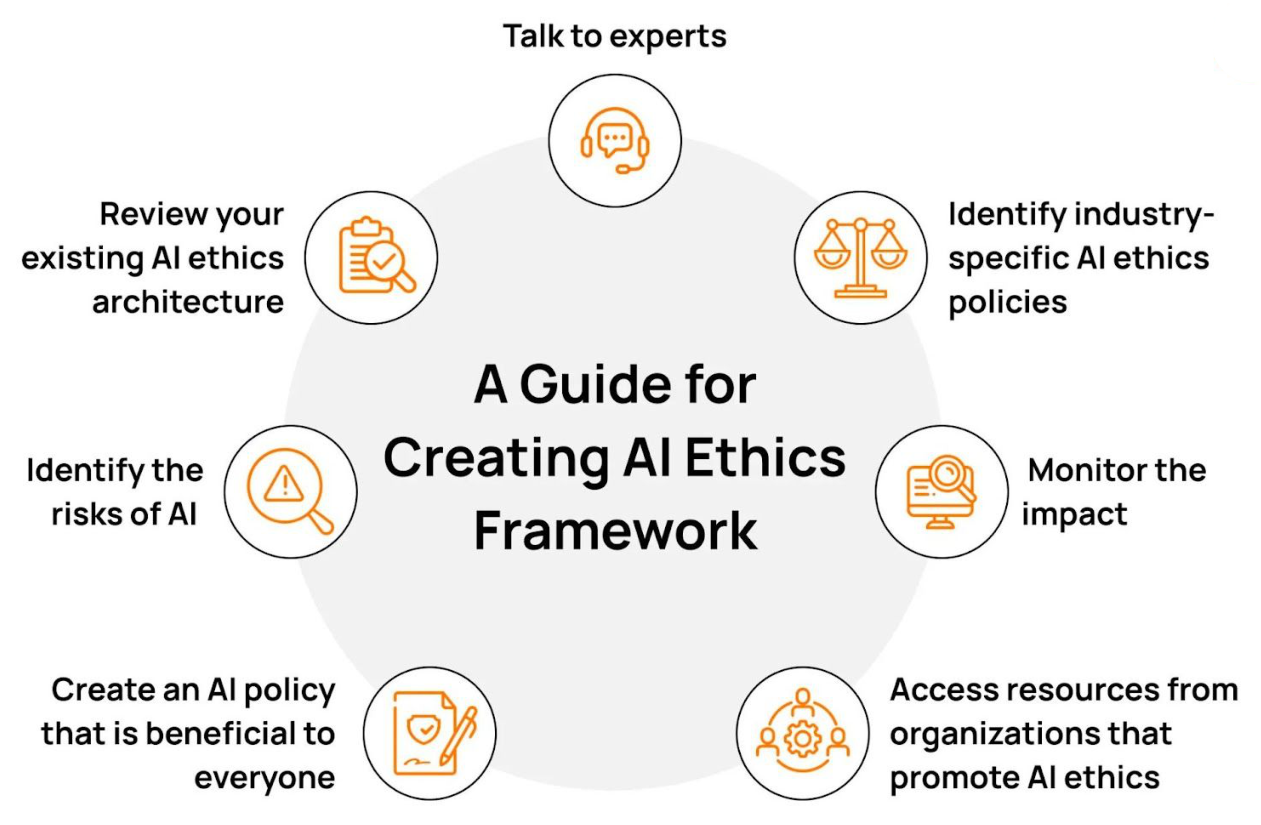
\includegraphics[width=0.8\textwidth,height=0.8\textheight,keepaspectratio]{assets/Lecture-10_Multimodal_NLP_Agentic_AI/slide_065.png}
\end{frame}

\begin{frame}{Ethics and Control}
  \begin{itemize}
    \item \textcolor{red}{Alignment:} Are agents acting in users' interests?
    \item \textcolor{red}{Accountability:} Who is responsible for AI actions?
    \item \textcolor{red}{Control:} Can humans override or audit decisions?
  \end{itemize}
  \vspace{1em}
  \textbf{Key Areas:}
  \begin{itemize}
    \item Fairness in multimodal data
    \item Bias amplification (vision + language)
    \item Transparency in decision-making
  \end{itemize}
\end{frame}
